\documentclass[a4paper]{article}

\def\npart {III}
\def\nterm {Lent}
\def\nyear {2017}
\def\nlecturer {B. P. Narayanan}
\def\ncourse {Ramsey Theory}
\def\nlectures {TT.9}

% Imports
\ifx \nextra \undefined
  \usepackage[pdftex,
    hidelinks,
    pdfauthor={Dexter Chua},
    pdfsubject={Cambridge Maths Notes: Part \npart\ - \ncourse},
    pdftitle={Part \npart\ - \ncourse},
  pdfkeywords={Cambridge Mathematics Maths Math \npart\ \nterm\ \nyear\ \ncourse}]{hyperref}
  \title{Part \npart\ - \ncourse}
\else
  \usepackage[pdftex,
    hidelinks,
    pdfauthor={Dexter Chua},
    pdfsubject={Cambridge Maths Notes: Part \npart\ - \ncourse\ (\nextra)},
    pdftitle={Part \npart\ - \ncourse\ (\nextra)},
  pdfkeywords={Cambridge Mathematics Maths Math \npart\ \nterm\ \nyear\ \ncourse\ \nextra}]{hyperref}

  \title{Part \npart\ - \ncourse \\ {\Large \nextra}}
\fi

\author{Lectured by \nlecturer \\\small Notes taken by Dexter Chua}
\date{\nterm\ \nyear}

\usepackage{alltt}
\usepackage{amsfonts}
\usepackage{amsmath}
\usepackage{amssymb}
\usepackage{amsthm}
\usepackage{booktabs}
\usepackage{caption}
\usepackage{enumitem}
\usepackage{fancyhdr}
\usepackage{graphicx}
\usepackage{mathtools}
\usepackage{microtype}
\usepackage{multirow}
\usepackage{pdflscape}
\usepackage{pgfplots}
\usepackage{siunitx}
\usepackage{tabularx}
\usepackage{tikz}
\usepackage{tkz-euclide}
\usepackage[normalem]{ulem}
\usepackage[all]{xy}

\pgfplotsset{compat=1.12}

\pagestyle{fancyplain}
\lhead{\emph{\nouppercase{\leftmark}}}
\ifx \nextra \undefined
  \rhead{
    \ifnum\thepage=1
    \else
      \npart\ \ncourse
    \fi}
\else
  \rhead{
    \ifnum\thepage=1
    \else
      \npart\ \ncourse\ (\nextra)
    \fi}
\fi
\usetikzlibrary{arrows}
\usetikzlibrary{decorations.markings}
\usetikzlibrary{decorations.pathmorphing}
\usetikzlibrary{positioning}
\usetikzlibrary{fadings}
\usetikzlibrary{intersections}
\usetikzlibrary{cd}

\newcommand*{\Cdot}{\raisebox{-0.25ex}{\scalebox{1.5}{$\cdot$}}}
\newcommand {\pd}[2][ ]{
  \ifx #1 { }
    \frac{\partial}{\partial #2}
  \else
    \frac{\partial^{#1}}{\partial #2^{#1}}
  \fi
}

% Theorems
\theoremstyle{definition}
\newtheorem*{aim}{Aim}
\newtheorem*{axiom}{Axiom}
\newtheorem*{claim}{Claim}
\newtheorem*{cor}{Corollary}
\newtheorem*{defi}{Definition}
\newtheorem*{eg}{Example}
\newtheorem*{fact}{Fact}
\newtheorem*{law}{Law}
\newtheorem*{lemma}{Lemma}
\newtheorem*{notation}{Notation}
\newtheorem*{prop}{Proposition}
\newtheorem*{thm}{Theorem}

\renewcommand{\labelitemi}{--}
\renewcommand{\labelitemii}{$\circ$}
\renewcommand{\labelenumi}{(\roman{*})}

\let\stdsection\section
\renewcommand\section{\newpage\stdsection}

% Strike through
\def\st{\bgroup \ULdepth=-.55ex \ULset}

% Maths symbols
\newcommand{\bra}{\langle}
\newcommand{\ket}{\rangle}

\newcommand{\N}{\mathbb{N}}
\newcommand{\Z}{\mathbb{Z}}
\newcommand{\Q}{\mathbb{Q}}
\renewcommand{\H}{\mathbb{H}}
\newcommand{\R}{\mathbb{R}}
\newcommand{\C}{\mathbb{C}}
\newcommand{\Prob}{\mathbb{P}}
\renewcommand{\P}{\mathbb{P}}
\newcommand{\E}{\mathbb{E}}
\newcommand{\F}{\mathbb{F}}
\newcommand{\cU}{\mathcal{U}}
\newcommand{\RP}{\mathbb{RP}}
\newcommand{\CP}{\mathbb{CP}}

\newcommand{\ph}{\,\cdot\,}

\DeclareMathOperator{\sech}{sech}
\DeclareMathOperator{\cosech}{cosech}
\DeclareMathOperator{\cosec}{cosec}

\DeclareMathOperator{\covol}{covol}
\DeclareMathOperator{\vol}{vol}

\let\Im\relax
\let\Re\relax
\DeclareMathOperator{\Im}{Im}
\DeclareMathOperator{\Re}{Re}
\DeclareMathOperator{\im}{im}
\DeclareMathOperator{\image}{image}
\DeclareMathOperator{\Ann}{Ann}

\DeclareMathOperator*{\res}{res}
\DeclareMathOperator{\Res}{Res}
\DeclareMathOperator{\Ind}{Ind}

\DeclareMathOperator{\tr}{tr}
\DeclareMathOperator{\diag}{diag}
\DeclareMathOperator{\rank}{rank}
\DeclareMathOperator{\card}{card}
\DeclareMathOperator{\spn}{span}
\DeclareMathOperator{\adj}{adj}

\DeclareMathOperator{\erf}{erf}
\DeclareMathOperator{\erfc}{erfc}

\DeclareMathOperator{\ord}{ord}
\DeclareMathOperator{\Sym}{Sym}

\DeclareMathOperator{\sgn}{sgn}
\DeclareMathOperator{\orb}{orb}
\DeclareMathOperator{\stab}{stab}
\DeclareMathOperator{\ccl}{ccl}

\DeclareMathOperator{\lcm}{lcm}
\DeclareMathOperator{\hcf}{hcf}

\DeclareMathOperator{\Int}{Int}
\DeclareMathOperator{\id}{id}

\DeclareMathOperator{\betaD}{beta}
\DeclareMathOperator{\gammaD}{gamma}
\DeclareMathOperator{\Poisson}{Poisson}
\DeclareMathOperator{\binomial}{binomial}
\DeclareMathOperator{\multinomial}{multinomial}
\DeclareMathOperator{\Bernoulli}{Bernoulli}
\DeclareMathOperator{\like}{like}

\DeclareMathOperator{\var}{var}
\DeclareMathOperator{\cov}{cov}
\DeclareMathOperator{\bias}{bias}
\DeclareMathOperator{\mse}{mse}
\DeclareMathOperator{\corr}{corr}

\DeclareMathOperator{\otp}{otp}
\DeclareMathOperator{\dom}{dom}

\DeclareMathOperator{\Root}{Root}
\DeclareMathOperator{\supp}{supp}
\DeclareMathOperator{\rel}{rel}
\DeclareMathOperator{\Hom}{Hom}
\DeclareMathOperator{\Aut}{Aut}
\DeclareMathOperator{\Gal}{Gal}
\DeclareMathOperator{\Mat}{Mat}
\DeclareMathOperator{\End}{End}
\DeclareMathOperator{\Char}{char}
\DeclareMathOperator{\ev}{ev}
\DeclareMathOperator{\St}{St}
\DeclareMathOperator{\Lk}{Lk}
\DeclareMathOperator{\disc}{disc}
\DeclareMathOperator{\Isom}{Isom}
\DeclareMathOperator{\length}{length}
\DeclareMathOperator{\energy}{energy}
\DeclareMathOperator{\area}{area}
\DeclareMathOperator{\Syl}{Syl}
\DeclareMathOperator{\cl}{cl}
\DeclareMathOperator{\fix}{fix}

\newcommand{\GL}{\mathrm{GL}}
\newcommand{\SL}{\mathrm{SL}}
\newcommand{\PGL}{\mathrm{PGL}}
\newcommand{\PSL}{\mathrm{PSL}}
\newcommand{\PSU}{\mathrm{PSU}}
\newcommand{\Or}{\mathrm{O}}
\newcommand{\SO}{\mathrm{SO}}
\newcommand{\U}{\mathrm{U}}
\newcommand{\SU}{\mathrm{SU}}

\renewcommand{\d}{\mathrm{d}}
\newcommand{\D}{\mathrm{D}}

\tikzset{->/.style = {decoration={markings,
                                  mark=at position 1 with {\arrow[scale=2]{latex'}}},
                      postaction={decorate}}}
\tikzset{<-/.style = {decoration={markings,
                                  mark=at position 0 with {\arrowreversed[scale=2]{latex'}}},
                      postaction={decorate}}}
\tikzset{<->/.style = {decoration={markings,
                                   mark=at position 0 with {\arrowreversed[scale=2]{latex'}},
                                   mark=at position 1 with {\arrow[scale=2]{latex'}}},
                       postaction={decorate}}}
\tikzset{->-/.style = {decoration={markings,
                                   mark=at position #1 with {\arrow[scale=2]{latex'}}},
                       postaction={decorate}}}
\tikzset{-<-/.style = {decoration={markings,
                                   mark=at position #1 with {\arrowreversed[scale=2]{latex'}}},
                       postaction={decorate}}}

\tikzset{circ/.style = {fill, circle, inner sep = 0, minimum size = 3}}
\tikzset{mstate/.style={circle, draw, blue, text=black, minimum width=0.7cm}}

\definecolor{mblue}{rgb}{0.2, 0.3, 0.8}
\definecolor{morange}{rgb}{1, 0.5, 0}
\definecolor{mgreen}{rgb}{0.1, 0.4, 0.2}
\definecolor{mred}{rgb}{0.5, 0, 0}

\def\drawcirculararc(#1,#2)(#3,#4)(#5,#6){%
    \pgfmathsetmacro\cA{(#1*#1+#2*#2-#3*#3-#4*#4)/2}%
    \pgfmathsetmacro\cB{(#1*#1+#2*#2-#5*#5-#6*#6)/2}%
    \pgfmathsetmacro\cy{(\cB*(#1-#3)-\cA*(#1-#5))/%
                        ((#2-#6)*(#1-#3)-(#2-#4)*(#1-#5))}%
    \pgfmathsetmacro\cx{(\cA-\cy*(#2-#4))/(#1-#3)}%
    \pgfmathsetmacro\cr{sqrt((#1-\cx)*(#1-\cx)+(#2-\cy)*(#2-\cy))}%
    \pgfmathsetmacro\cA{atan2(#2-\cy,#1-\cx)}%
    \pgfmathsetmacro\cB{atan2(#6-\cy,#5-\cx)}%
    \pgfmathparse{\cB<\cA}%
    \ifnum\pgfmathresult=1
        \pgfmathsetmacro\cB{\cB+360}%
    \fi
    \draw (#1,#2) arc (\cA:\cB:\cr);%
}
\newcommand\getCoord[3]{\newdimen{#1}\newdimen{#2}\pgfextractx{#1}{\pgfpointanchor{#3}{center}}\pgfextracty{#2}{\pgfpointanchor{#3}{center}}}

\def\Xint#1{\mathchoice
   {\XXint\displaystyle\textstyle{#1}}%
   {\XXint\textstyle\scriptstyle{#1}}%
   {\XXint\scriptstyle\scriptscriptstyle{#1}}%
   {\XXint\scriptscriptstyle\scriptscriptstyle{#1}}%
   \!\int}
\def\XXint#1#2#3{{\setbox0=\hbox{$#1{#2#3}{\int}$}
     \vcenter{\hbox{$#2#3$}}\kern-.5\wd0}}
\def\ddashint{\Xint=}
\def\dashint{\Xint-}


\begin{document}
\maketitle
{\small
\setlength{\parindent}{0em}
\setlength{\parskip}{1em}

What happens when we cut up a mathematical structure into many `pieces' ? How big must the original structure be in order to guarantee that at least one of the pieces has a specific property of interest? These are the kinds of questions at the heart of Ramsey theory. A prototypical result in the area is van der Waerden's theorem, which states that whenever we partition the natural numbers into finitely many classes, there is a class that contains arbitrarily long arithmetic progressions.

The course will cover both classical material and more recent developments in the subject. Some of the classical results that I shall cover include Ramsey's theorem, van der Waerden's theorem and the Hales--Jewett theorem; I shall discuss some applications of these results as well. More recent developments that I hope to cover include the properties of non-Ramsey graphs, topics in geometric Ramsey theory, and finally, connections between Ramsey theory and topological dynamics. I will also indicate a number of open problems.

\subsubsection*{Pre-requisites}
There are almost no pre-requisites and the material presented in this course will, by and large, be self-contained. However, students familiar with the basic notions of graph theory and point-set topology are bound to find the course easier.
}
\tableofcontents

\section{Graph Ramsey theory}
\subsection{Infinite graphs}
We start by laying out some notations and definitions.
\begin{notation}
  $\N$ does not include $0$.
\end{notation}

\begin{notation}
  For a set $X$, we write $X^{(r)}$\index{$X^{(r)}$} for the subsets of $X$ of size $r$.
\end{notation}
\begin{notation}
  We write $\N$\index{$\N$} for the natural numbers, not including $0$, and $[n]$\index{$[n]$} for $\{1, 2, \cdots, n\}$.
\end{notation}

\begin{defi}[Graph]\index{graph}
  A graph $G$ is a pair $(V, E)$, where $E \subseteq V^{(2)}$.
\end{defi}
When writing edges $\{i. j\} \in \N^{(2)}$, we will simply write it as $ij$. Moreover, we always assume that we have $i < j$.

\begin{defi}[$k$-colouring]\index{$k$-colouring}\index{colouring}
  A $k$-colouring of a set $X$ is a map $c: X \to [k]$.
\end{defi}

\begin{defi}[Monochromatic set]\index{monochromatic set}
  Let $X$ be a set with a $k$-colouring. We say a subset $Y \subseteq X$ is \emph{monochromatic} if the colouring restricted to $Y$ is constant.
\end{defi}
Much of Ramsey theory is about the following question --- we have a set $X$ that has some nice structures. If we $k$-colour this set $X$, can we find a monochromatic subset of $X$ that retains some of this structure?

The first question we ask is about graphs:
\begin{question}
  If $\N^{(2)}$ is $k$-coloured, can we find a complete infinite subgraph that is monochromatic? In other words, is there an infinite subset $X \subseteq \N$ such that $X^{(2)} \subseteq \N^{(2)}$ is monochromatic?
\end{question}

We try to look at some examples:
\begin{eg}
  Suppose we had the colouring $c: \N^{(2)} \to \{\mathrm{red}, \mathrm{blue}\}$ by
  \[
    c(ij) =
    \begin{cases}
      \mathrm{red} & i + j \text{ is even}\\
      \mathrm{blue} & i + j \text{ is odd}
    \end{cases}.
  \]
  Then we can pick $X = \{2, 4, 6, 8, \cdots \}$, and this is an infinite monochromatic set.
\end{eg}

\begin{eg}
  Consider $c: \N^{(2)} \to \{0, 1, 2\}$, where
  \[
    c(ij) = \max \{n: 2^n \mid i + j\} \bmod 3
  \]
  In this case, taking $X = \{8, 8^2, 8^3, \cdots\}$ gives an infinite monochromatic set of colour $0$.
\end{eg}

\begin{eg}
  Let $c: \N^{(2)} \to \{\mathrm{red}, \mathrm{blue}\}$ by
  \[
    c(ij) =
    \begin{cases}
      \mathrm{red} & i + j\text{ has an even number of distinct prime factors}\\
      \mathrm{blue} & \mathrm{otherwise}
    \end{cases}
  \]
\end{eg}
It is in fact an open problem to find an explicit infinite monochromatic set for this colouring, or even for which colour do we have an infinite monochromatic set. However, we can prove that such a set must exist!

\begin{thm}[Ramsey's theorem]\index{Ramsey's theorem}
  Whenever we $k$-colour $\N^{(2)}$, there exists an infinite monochromatic set $X$, ie. given any map $c: \N^{(2)} \to [k]$, there exists a subset $X \subseteq \N$ such that $X$ is infinite and $c|_{X^{(2)}}$ is a constant function.
\end{thm}

\begin{proof}
  Pick an arbitrary point $a_1 \in \N$. Then by the pigeonhole principle, there must exist an infinite set $\mathcal{B}_1 \subseteq \N \setminus \{a_1\}$ such that all the $a_1\mdash \mathcal{B}_1$ edges (ie. edges of the form $(a_1, b_1)$ with $b_1 \in \mathcal{B}_1$) are of the same colour $c_1$.

  Now again arbitrarily pick an element $a_2 \in \mathcal{B}_1$. Again, we find some $\mathcal{B}_2 \subseteq \mathcal{B}_1$ such that all $a_2$-$\mathcal{B}_2$ edges are the same colour $c_2$. We proceed inductively.
  \begin{center}
    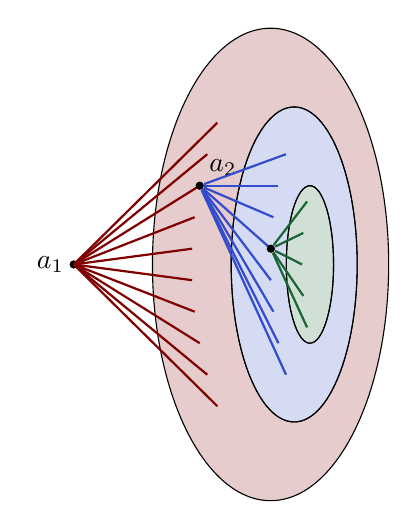
\begin{tikzpicture}
      \draw [fill opacity=0.2, fill=mred] ellipse (1.5 and 3);

      \draw [fill=white] (0.3, 0) ellipse (0.8 and 2);
      \draw [fill opacity=0.2, fill=mblue] (0.3, 0) ellipse (0.8 and 2);
      \draw [fill=white] (0.5, 0) ellipse (0.3 and 1);
      \draw [fill opacity=0.2, fill=mgreen] (0.5, 0) ellipse (0.3 and 1);

      \node [circ] at (-2.5, 0) {};
      \node [left] at (-2.5, 0) {$a_1$};

      \foreach \y in {1.8, 1.4, 1, 0.6, 0.2, -0.2, -0.6, -1, -1.4, -1.8} {
        \pgfmathsetmacro{\x}{-1 + 0.1 * abs(\y)^2};
        \draw [mred, thick] (-2.5, 0) -- (\x, \y) ;
      }
      \node [circ] (a2) at (-0.9, 1) {};
      \node [anchor=south west] at (a2) {$a_2$};
      \foreach \y in {1.4, 1, 0.6, 0.2, -0.2, -0.6, -1, -1.4} {
        \pgfmathsetmacro{\x}{0.1 * abs(\y)^2};
        \draw [mblue, thick] (a2) -- (\x, \y) ;
      }
      \node [circ] (a3) at (0.004, 0.2) {};
      \foreach \y in {0.8, 0.4, 0, -0.4, -0.8} {
        \pgfmathsetmacro{\x}{0.4 + 0.1 * abs(\y)^2};
        \draw [mgreen, thick] (a3) -- (\x, \y) ;
      }
    \end{tikzpicture}
  \end{center}
  We obtain a sequence $\{a_1, a_2, \cdots\}$ and a sequence of colours $\{c_1, c_2, \cdots\}$ such that $c(a_i a_j) = c_i$, for $i < j$.

  Now again by the pigeonhole principle, since there are finitely many colours, there exists an infinite subsequence $c_{i_1}, c_{i_2}, \cdots$ that is constant. Then $a_{i_1}, a_{i_2}, \cdots$ is an infinite monochromatic set, since all edges are of the colour $c_{i_1} = c_{i_2} = \cdots$. So we are done.
\end{proof}
This proof exhibits many common themes we will see in the different Ramsey theory proofs we will later do. The first is that the proof is highly non-constructive. Not only does it not give us the infinite monochromatic set; it doesn't even tell us what the colour is.

Another feature of the proof is that we did not obtain the infinite monochromatic set in one go. Instead, we had to first pass through that intermediate structure, and then obtain an infinite monochromatic set from that. In future proofs, we might have to go through \emph{many} passes, instead of just two.

This theorem looks rather innocuous, but it has many interesting applications.
\begin{cor}[Bolzano-Weierstrass theorem]
  Let $(x_i)_{i \geq 0}$ be a bounded sequence of real numbers. Then it has a convergent subsequence.
\end{cor}

\begin{proof}
  We define a colouring $c: \N^{(2)} \to \{\uparrow, \downarrow\}$, where
  \[
    c(ij) =
    \begin{cases}
      \uparrow & x_i < x_j\\
      \downarrow & x_j \leq x_i
    \end{cases}
  \]
  Then Ramsey's theorem gives us an infinite monochromatic set, which is the same as a monotone subsequence. Since this is bounded, it must convergence.
\end{proof}

With a very similar technique, we can prove that we can do this for $\N^{(r)}$ for any $r$, and not just $\N^{(2)}$.
\begin{thm}[Ramsey's theorem for $r$ sets]\index{Ramsey's theorem!for $r$ sets}
  Whenever $\N^{(r)}$ is $k$-coloured, there exists an infinite monochromatic set, ie. for any $c: \N^{(r)} \to [k]$, there exists an infinite $X \subseteq \N$ such that $c|_{X^{(r)}}$ is constant.
\end{thm}

We can again try some concrete examples:
\begin{eg}
  We define $c: \N^{(3)} \to \{\mathrm{red}, \mathrm{blue}\}$ by
  \[
    c(ijk) =
    \begin{cases}
      \mathrm{red} & i \mid j + k\\
      \mathrm{blue} & \mathrm{otherwise}
    \end{cases}
  \]
  Then $X = \{2^0, 2^1, 2^2, \cdots\}$ is an infinite monochromatic set.
\end{eg}

\begin{proof}
  We induct on $r$. This is trivial when $r = 1$. Assume $r > 1$. We fix $a_1 \in \N$. We induce a $k$-colouring $c_1$ of $(\N \setminus \{a_1\})^{(r - 1)}$ by
  \[
    c_1(F) = c(F \cup \{a_1\}).
  \]
  By induction, there exists an infinite $B_1 \subseteq \N \setminus \{a_1\}$ such that $B_1$ is monochromatic for $c_1$, ie. all $a_1\mdash B_1$ $r$-sets have the same colour $c_1$.

  We proceed inductively as before. We get $a_1, a_2, a_3, \cdots$ and colours $c_1, c_2, \cdots$ etc. such that for any $r$-set $F$ contained in $\{a_1, a_2, \cdots\}$, we have $c(F) = c_{\min F}$.

  Then again, there exists $c_{i_1}, c_{i_2}, c_{i_3}, \cdots$ all identical, and our monochromatic set is $\{a_{i_1}, a_{i_2}, a_{i_3}, \cdots\}$.
\end{proof}


Now a natural question to ask is --- what happens when we have infinitely many colours? Clearly an infinite monochromatic subset cannot be guaranteed, because we can just colour all edges with different colours.

The natural compromise is to ask if we can find an $X$ such that \emph{either} $c|_{X}$ is monochromatic, \emph{or} $c|_{X}$ is injective. After a little thought, we realize this is also impossible. We can construct a colouring on $\N^{(2)}$ as follows: we first colour all edges that involve $1$ with the colour $1$, then all edges that involve $2$ with the colour $2$ etc:
\begin{center}
  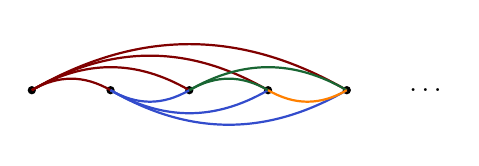
\begin{tikzpicture}
    \foreach \x in {1, 2, 3, 4, 5} {
      \node [circ] at (\x, 0) {};
    }

    \foreach \x in {2, 3, 4, 5} {
      \draw (1, 0) edge [bend left, mred, thick] (\x, 0);
    }
    \foreach \x in {3, 4, 5} {
      \draw (2, 0) edge [bend right, mblue, thick] (\x, 0);
    }
    \foreach \x in {4, 5} {
      \draw (3, 0) edge [bend left, mgreen, thick] (\x, 0);
    }
    \foreach \x in {5} {
      \draw (4, 0) edge [bend right, morange, thick] (\x, 0);
    }
    \node at (6, 0) {$\ldots$};
  \end{tikzpicture}
\end{center}
It is easy to see that we cannot find an infinite monochromatic subset or an infinite subset with all edges of different colours.

However, this counterexample we came up with still has a high amount of structure --- the colour of the edges are uniquely determined by the first element. It turns out this is the only missing piece (plus the obvious dual case).

With this, we can answer our previous question:
\begin{thm}[Canonical Ramsey theorem]\index{canonical Ramsey theorem}\index{Ramsey theorem!canonical}
  For any $c: \N^{(2)} \to \N$, there exists an infinite $X \subseteq \N$ such that one of the following hold:
  \begin{enumerate}
    \item $c|_{X^{(2)}}$ is constant.
    \item $c|_{X^{(2)}}$ is injective.
    \item $c(ij) = c(k\ell)$ iff $i = k$ for all $i, j, k, \ell \in X$.
    \item $c(ij) = c(k\ell)$ iff $j = \ell$ for all $i, j, k, \ell \in X$.
  \end{enumerate}
\end{thm}
Recall that when we write $ij$, we always implicitly assume $i < j$, so that (iii) and (iv) make sense.

In previous proofs, we only had to go through two passes to get the desired set. This time we will need more.
\begin{proof}
  Consider the following colouring of $X^{(4)}$: let $c_1$ be a $2$-colouring
  \[
    c_1(ijk\ell) =
    \begin{cases}
      \mathtt{SAME} & c(ij) = c(k\ell)\\
      \mathtt{DIFF} & \mathrm{otherwise}
    \end{cases}
  \]
  \begin{center}
    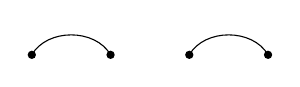
\begin{tikzpicture}
      \foreach \x in {0, 1, 2, 3} {
        \node [circ] at (\x, 0) {};
      }
      \draw (0, 0) edge [out=60, in=120] (1, 0);
      \draw (2, 0) edge [out=60, in=120] (3, 0);
    \end{tikzpicture}
  \end{center}
  Then we know there is some infinite monochromatic set $X_1 \subseteq \N$ for $c_1$. If $X_1$ is coloured $\mathtt{SAME}$, then we are done. Indeed, for any pair $ij$ and $i'j'$ in $X_1$, we can pick some huge $k, \ell$ such that $j, j' < k < \ell$, and then
  \[
    c(ij) = c(k\ell) = c(i'j')
  \]
  as we know $c_1(ijk\ell) = c_1(i'j'k\ell) = \mathtt{SAME}$.

  What if $X_1$ is coloured $\mathtt{DIFF}$? We next look at what happens when we have edges that are nested each other. We define $c_2: X_1^{(4)} \to \{\mathtt{SAME}, \mathtt{DIFF}\}$ defined by
  \[
    c_2(ijk\ell) =
    \begin{cases}
      \mathtt{SAME} & c(i\ell) = c(jk)\\
      \mathtt{DIFF} & \mathrm{otherwise}
    \end{cases}
  \]
  \begin{center}
    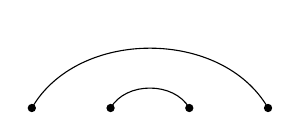
\begin{tikzpicture}
      \foreach \x in {0, 1, 2, 3} {
        \node [circ] at (\x, 0) {};
      }
      \draw (0, 0) edge [out=60, in=120] (3, 0);
      \draw (1, 0) edge [out=60, in=120] (2, 0);
    \end{tikzpicture}
  \end{center}
  Again, we can find an infinite monochromatic subset $X_2 \subseteq X_1$ with respect to $c_2$.

  We now note that $X_2$ cannot be coloured $\mathtt{SAME}$. Indeed, we can just look at
  \begin{center}
    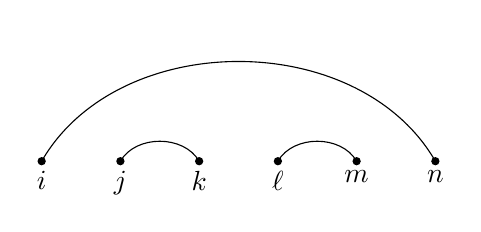
\begin{tikzpicture}
      \foreach \x/\y in {0/i, 1/j, 2/k, 3/\ell, 4/m, 5/n} {
        \node [circ] at (\x, 0) {};
        \node [below] at (\x, 0) {$\y$};
      }
      \draw (0, 0) edge [out=60, in=120] (5, 0);
      \draw (1, 0) edge [out=60, in=120] (2, 0);
      \draw (3, 0) edge [out=60, in=120] (4, 0);
    \end{tikzpicture}
  \end{center}
  So if $X_2$ were $\mathtt{SAME}$, we would have
  \[
    c(\ell m) = c(in) = c(jk),
  \]
  which is impossible since $X_1$ is coloured $\mathtt{DIFF}$ under $c_1$.

  So $X_2$ is $\mathtt{DIFF}$. Now consider $c_3: X_2^{(4)} \to \{\mathtt{SAME}, \mathtt{DIFF}\}$ given by
  \[
    c_3(ijk\ell) =
    \begin{cases}
      \mathtt{SAME} & c(ik) = c(j\ell)\\
      \mathtt{DIFF} & \mathrm{otherwise}
    \end{cases}
  \]
  \begin{center}
    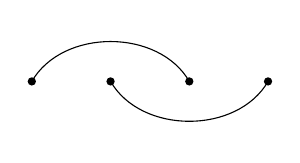
\begin{tikzpicture}
      \foreach \x in {0, 1, 2, 3} {
        \node [circ] at (\x, 0) {};
      }
      \draw (0, 0) edge [out=60, in=120] (2, 0);
      \draw (1, 0) edge [out=-60, in=-120] (3, 0);
    \end{tikzpicture}
  \end{center}
  Again find an infinite monochromatic subset $X_3 \subseteq X_2$ for $c_3$. Then $X_3$ cannot be $\mathtt{SAME}$, this time using the following picture:
   \begin{center}
    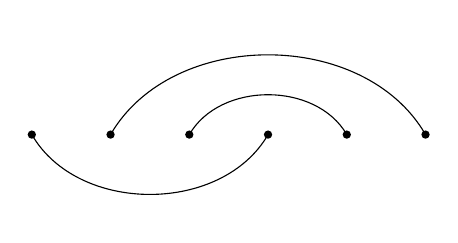
\begin{tikzpicture}
      \foreach \x/\y in {0, 1, 2, 3, 4, 5} {
        \node [circ] at (\x, 0) {};
      }
      \draw (0, 0) edge [out=-60, in=-120] (3, 0);
      \draw (1, 0) edge [out=60, in=120] (5, 0);
      \draw (2, 0) edge [out=60, in=120] (4, 0);
    \end{tikzpicture}
  \end{center}
  contradicting the fact that $c_2$ is $\mathtt{DIFF}$. So we know $X_3$ is $\mathtt{DIFF}$.

  We have now have ended up in this set $X_3$ such that if we have any two pairs of edges with different end points, then they must be different.

  We now want to look at cases where things share a vertex. Consider $c_4: X_3^{(3)} \to \{\mathtt{SAME}, \mathtt{DIFF}\}$ given by
  \[
    c_4(ijk) =
    \begin{cases}
      \mathtt{SAME} & c(ij) = c(jk)\\
      \mathtt{DIFF} & \mathrm{otherwise}
    \end{cases}
  \]
  \begin{center}
    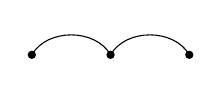
\begin{tikzpicture}
      \foreach \x in {0, 1, 2} {
        \node [circ] at (\x, 0) {};
      }
      \draw (0, 0) edge [out=60, in=120] (1, 0);
      \draw (1, 0) edge [out=60, in=120] (2, 0);
    \end{tikzpicture}
  \end{center}
  Let $X_4 \subseteq X_3$ be an infinite monochromatic set for $c_4$. Now $X_4$ cannot be coloured $\mathtt{SAME}$, using the following picture:
  \begin{center}
    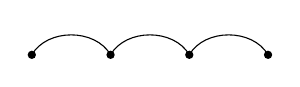
\begin{tikzpicture}
      \foreach \x in {0, 1, 2, 3} {
        \node [circ] at (\x, 0) {};
      }
      \draw (0, 0) edge [out=60, in=120] (1, 0);
      \draw (1, 0) edge [out=60, in=120] (2, 0);
      \draw (2, 0) edge [out=60, in=120] (3, 0);
    \end{tikzpicture}
  \end{center}
  which contradicts the fact that $c_1$ is $\mathtt{DIFF}$. So we know $X_4$ is also coloured $\mathtt{DIFF}$ under $c_4$.

  We are almost there. We need to deal with edges that nest in the sense of (iii) and (iv). We look at $c_5: X_4^{(3)} \to \{\mathtt{LSAME}, \mathtt{LDIFF}\}$ given by
  \[
    c_5(ijk) =
    \begin{cases}
      \mathtt{LSAME} & c(ij) = c(ik)\\
      \mathtt{LDIFF} & \mathrm{otherwise}
    \end{cases}
  \]
   \begin{center}
    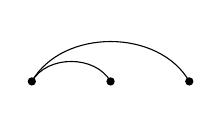
\begin{tikzpicture}
      \foreach \x in {0, 1, 2} {
        \node [circ] at (\x, 0) {};
      }
      \draw (0, 0) edge [out=60, in=120] (1, 0);
      \draw (0, 0) edge [out=60, in=120] (2, 0);
    \end{tikzpicture}
  \end{center}
  Again we find $X_5 \subseteq X_4$, an infinite monochromatic set for $c_5$. We don't separate into cases yet, because we know both cases are possible, but move on to classify the right case as well. Define $c_6: X_5^{(3)} \to \{\mathtt{RSAME}, \mathtt{RDIFF}\}$ given by
  \[
    c_5(ijk) =
    \begin{cases}
      \mathtt{RSAME} & c(ik) = c(jk)\\
      \mathtt{RDIFF} & \mathrm{otherwise}
    \end{cases}
  \]
   \begin{center}
    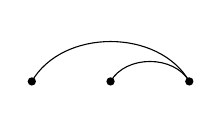
\begin{tikzpicture}
      \foreach \x in {0, 1, 2} {
        \node [circ] at (\x, 0) {};
      }
      \draw (1, 0) edge [out=60, in=120] (2, 0);
      \draw (0, 0) edge [out=60, in=120] (2, 0);
    \end{tikzpicture}
  \end{center}
  Let $X_6 \subseteq X_5$ be an infinite monochromatic subset under $c_5$.

  As before, we can check that it is impossible to get both $\mathtt{LSAME}$ and $\mathtt{RSAME}$, using the following picture:
  \begin{center}
    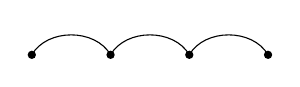
\begin{tikzpicture}
      \foreach \x in {0, 1, 2, 3} {
        \node [circ] at (\x, 0) {};
      }
      \draw (0, 0) edge [out=60, in=120] (1, 0);
      \draw (1, 0) edge [out=60, in=120] (2, 0);
      \draw (2, 0) edge [out=60, in=120] (3, 0);
    \end{tikzpicture}
  \end{center}
  contradicting $c_4$ being $\mathtt{DIFF}$.

  Then the remaining cases $(\mathtt{LDIFF}, \mathtt{RDIFF})$, $(\mathtt{LSAME}, \mathtt{RDIFF})$ and $(\mathtt{RDIFF}, \mathtt{LSAME})$ corresponds to the cases (ii), (iii) and (iv).
\end{proof}
Note that we could this theorem in one pass only, instead of six, by considering a much more complicated colouring $(c_1, c_2, c_3, c_4, c_5, c_6)$ with values in
\[
  \{\mathtt{SAME}, \mathtt{DIFF}\}^4 \times \{\mathtt{LSAME}, \mathtt{LDIFF}\} \times \{\mathtt{RSAME}, \mathtt{RDIFF}\},
\]
but we still have to do the same analysis and it just complicates matters more.

There is a generalization of this to $r$-sets. One way we can rewrite the theorem is to say that the colour is uniquely determined by some subset of the vertices. The cases (i), (ii), (iii), (iv) correspond to no vertices, all vertices, first vertex, and second vertex respectively. Then for $r$-sets, we have $2^r$ possibilities, one for each subset of the $r$-coordinates.

\begin{thm}[Higher dimensional canonical Ramsey theorem]\index{higher dimensional canonical Ramsey theorem}\index{canonical Ramsey theorem!!higher dimensional}\index{Ramsey theorem!higher dimensional, canonical}
  Let $c: \N^{(r)} \to \N$ be a colouring. Then there exists $D \subseteq [r]$ and an infinite subset $X \subseteq \N$ such that for all $x \not= y \in X^{(r)}$, we have $c(x) = c(y)$ iff $\{i: x_i = y_i\} = D$, where $x = \{x_1 < x_2 < \cdots < x_r\}$ (and similarly for $y$).
\end{thm}

\subsection{Finite graphs}
Before we begin, we note some definitions. Recall again that a graph $G$ is a pair $(V, E)$ where $E \subseteq V^{(2)}$.
\begin{eg}
  The \term{path graph} on $n$ vertices \term{$P_n$} is
  \begin{center}
    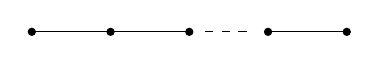
\begin{tikzpicture}
      \draw (0, 0) node [circ] {} -- (1, 0) node [circ] {} -- (2, 0) node [circ] {};

      \draw [dashed] (2.2, 0) -- (2.8, 0);

      \draw (3, 0) node [circ] {} -- (4, 0) node [circ] {};
    \end{tikzpicture}
  \end{center}
  We can write
  \[
    V = [n],\quad E = \{12, 23, 34, \cdots, (n-1)n\}.
  \]
\end{eg}

\begin{eg}
  The $n$-cycle \term{$C_n$} is
  \[
    V = [n],\quad E = \{12, 23, \cdots, (n-1)n, 1n\}.
  \]
  \begin{center}
    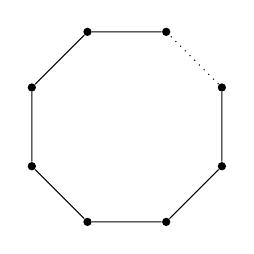
\begin{tikzpicture}

      \node [circ] (0) at (1, 0) {};
      \node [circ] (1) at (0, 0) {};
      \node [circ] (2) at (-0.707, -0.707) {};
      \node [circ] (3) at (-0.707, -1.707) {};
      \node [circ] (4) at (0, -2.414) {};
      \node [circ] (5) at (1, -2.414) {};
      \node [circ] (6) at (1.707, -1.707) {};
      \node [circ] (7) at (1.707, -0.707) {};

      \draw (0) -- (1) -- (2) -- (3) -- (4) -- (5) -- (6) -- (7);
      \draw [dotted] (7) -- (0);
    \end{tikzpicture}
  \end{center}
\end{eg}

Finally, we have
\begin{eg}
  The \term{complete graph} \term{$V_n$} on $n$ vertices is
  \[
    V = [n], E = V^{(2)}.
  \]
  \begin{center}
    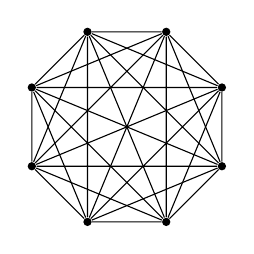
\begin{tikzpicture}

      \node [circ] (0) at (1, 0) {};
      \node [circ] (1) at (0, 0) {};
      \node [circ] (2) at (-0.707, -0.707) {};
      \node [circ] (3) at (-0.707, -1.707) {};
      \node [circ] (4) at (0, -2.414) {};
      \node [circ] (5) at (1, -2.414) {};
      \node [circ] (6) at (1.707, -1.707) {};
      \node [circ] (7) at (1.707, -0.707) {};

      \draw (0) -- (1) -- (2) -- (3) -- (4) -- (5) -- (6) -- (7) -- (0);
      \draw (0) -- (2) -- (4) -- (6) -- (0);
      \draw (1) -- (3) -- (5) -- (7) -- (1);
      \draw (0) -- (3) -- (6) -- (1) -- (4) -- (7) -- (2) -- (5) -- (0);
      \draw (0) -- (4);
      \draw (1) -- (5);
      \draw (2) -- (6);
      \draw (3) -- (7);
    \end{tikzpicture}
  \end{center}
\end{eg}
Our previous Ramsey theorem can be said as saying given an infinite complete graph $K_\N$ with a colouring, there is an infinite monochromatic complete subgraph. Obviously, our initial graph had to be infinite for the result to hold. But we can ask another question --- how big does our graph have to be to guarantee a complete monochromatic subgraph of size $n$?

In this section, we will usually restrict to $2$ colours. Everything we say will either be trivially be generalizable to more colours, or we have no idea how to do so. It is an exercise for the reader to figure out which it is.
\begin{defi}[Ramsey number]\index{Ramsey number}\index{$R(n)$}\index{$R(K_n)$}
  We let $R(n) = R(K_n)$ to be the smallest $N \in \N$ whenever we red-blue colour the edges of $K_N$, then there is a monochromatic copy of $K_n$.
\end{defi}

It is not immediately obvious that $R(n)$ has to exist, ie. it is a finite number. It turns out we can easily prove this from the infinite Ramsey theorem.
\begin{thm}[Finite Ramsey theorem]\index{finite Ramsey theorem}
  For all $n$, we have $R(n) < \infty$.
\end{thm}

\begin{proof}
  Suppose not. Let $n$ be such that $R(n) = \infty$. Then for any $m \geq n$, there is a $2$-colouring $c_m$ of $K_m = [m]^{(2)}$ such that there is no monochromatic set of size $n$.

  We want to use these colourings to build up a colouring of $\N^{(2)}$ with no monochromatic set of size $n$. We want to say we take the ``limit'' of these colourings, but what does this mean? To do so, we need these colourings to be nested.

  By the pigeonhole principle, there exists an infinite set $M_1 \subseteq \N$ and some fixed $2$-colouring $d_n$ of $[n]$ such that $c_m|_{[n]^{(2)}} = d_n$ for all $m \in M_1$.

  Similarly, there exists an infinite $M_2 \subseteq M_1$ such that $c_m|_{[n + 1]^{(2)}} = d_{n + 1}$ for $m \in M_2$, again for some $2$-colouring $d_{n + 1}$ of $[n + 1]$. We repeat this over and over again. Then we get a sequence $d_n, d_{n + 1}, \cdots$ of colourings such that $d_i$ is a $2$-colouring of $[i]^{(2)}$ without a monochromatic $K_n$, and further for $i < j$, we have
  \[
    d_j|_{[i]^{(2)}} = d_i.
  \]
  We then define a $2$-colouring $c$ of $\N^{(2)}$ by
  \[
    c(ij) = d_m(ij)
  \]
  for any $m > i, j$. Clearly, there exists no monochromatic $K_n$ in $c$, as any $K_n$ is finite. This massively contradicts the infinite Ramsey theorem.
\end{proof}

There are other ways of obtaining the finite Ramsey theorem from the infinite one. For example, we can use the compactness theorem for first order logic.
\begin{proof}
  Suppose $R(n) = \infty$. Consider the theory with proposition letters $p_{ij}$ for each $ij \in \N^{(2)}$. We will think of the edge $ij$ as red if $p_{ij} = \top$, and blue if $p_{ij} = \bot$. For each subset of $\N$ of size $n$, we add in the axiom that says that set is not monochromatic.

  Then given any finite subset of the axioms, it mentions only finitely many subsets of $\N$. Suppose it mentions vertices only up to $m \in \N$. Then by assumption, there is a $2$-colouring of $[m]^{(2)}$ with no monochromatic subset of size $n$. So by assigning $p_{ij}$ accordingly (and randomly assigning the remaining ones), we have found a model of this finite subtheory. Thus every finite fragment of the theory is consistent. Hence the original theory is consistent. So there is a model, ie. a colouring of $\N^{(2)}$ with no monochromatic subset.

  This contradicts the infinite Ramsey theorem.
\end{proof}

Similarly, we can do it by compactness of the space $\{1, 2\}^\N$ endowed with metric
\[
  d(f, g) = \frac{1}{2^n}\text{ if } n = \min \{i: f_i \not= g_i\}.
\]
By Tychonoff theorem, we know this is compact, and we can deduce the theorem from this. % how?

While these theorems save work by reusing the infinite Ramsey theorem, it is highly non-constructive. It is useless if we want to obtain an actual bound on $R(n)$. We now go back and see what we did when we proved the infinite Ramsey theorem.

We randomly pick a point $a_1$. Then there are some things that are connected by red to it, and others connected by blue:
\begin{center}
  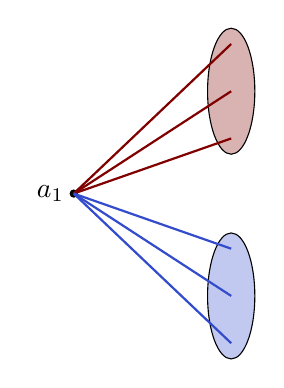
\begin{tikzpicture}
    \node [circ] {};
    \node [left] {$a_1$};

    \draw [fill opacity=0.3, fill=mred] (2, 1.3) ellipse (0.3 and 0.8);
    \draw [fill opacity=0.3, fill=mblue] (2, -1.3) ellipse (0.3 and 0.8);

    \draw [thick, mred] (0, 0) -- (2, 1.9);
    \draw [thick, mred] (0, 0) -- (2, 1.3);
    \draw [thick, mred] (0, 0) -- (2, 0.7);

    \draw [thick, mblue] (0, 0) -- (2, -1.9);
    \draw [thick, mblue] (0, 0) -- (2, -1.3);
    \draw [thick, mblue] (0, 0) -- (2, -0.7);
  \end{tikzpicture}
\end{center}
Next we randomly pick a point in one of the red or blue sets, and try to move on from there. Suppose we landed in the red one. Now note that if we find a blue $K_n$ in the red set, then we are done. But on the other hand, we only need a red $K_{n - 1}$, and not a full blown $K_n$. When we moved to this red set, the problem is no longer symmetric.

Thus, to figure out a good bound, it is natural to consider an asymmetric version of the problem.
\begin{defi}[Off-diagonal Ramsey number]\index{off-diagonal Ramsey number}\index{Ramsey number!off-diagonal}\index{$R(n, m)$}\index{$R(K_n, K_m)$}
  We define $R(n, m) = R(K_n, K_m)$ to be the minimum $N \in \N$ such that whenever we red-blue colour the edges of $K_N$, we either get a red $K_n$ or a blue $K_m$.
\end{defi}

Clearly we have
\[
  R(n, m) \leq R(\max\{n, m\}).
\]
In particular, they are finite. Once we make this definition, it is easy to find a bound on $R$.
\begin{thm}
  We have
  \[
    R(n, m) \leq R(n - 1, m) + R(n, m - 1).
  \]
  for all $n, m \in \N$. Consequently, we have
  \[
    R(n, m) \leq \binom{n + m - 1}{n - 2}.
  \]
\end{thm}

\begin{proof}
  We induct on $n + m$. It is clear that
  \[
    R(1, n) = R(n, 1) = 1,\quad R(n, 2) = R(2, n) = n
  \]
  Now suppose $N \geq R(n - 1, m) + R(n, m - 1)$. Consider any red-blue colouring of $K_N$ and any vertex $v \in V(K_n)$. We write
  \[
    v(K_n) \setminus \{v\} = A \cup B,
  \]
  where each vertex $A$ is joined by a red edge to $v$, and each vertex in $B$ is joined by a blue edge to $v$. Then
  \[
    |A| + |B| \geq N - 1 \geq R(n - 1, m) + R(n, m - 1) - 1.
  \]
  It follows that either $|A| \geq R(n - 1, m)$ or $|B| \geq R(n, m - 1)$. We wlog it is the former. Then by definition of $R(n - 1, m)$, we know $A$ contains either a blue copy of $K_m$ or a red copy of $K_{n - 1}$. In the first case, we are done, and in the second case, we just add $v$ to the red $K_{n - 1}$.

  The last formula is just a straightforward property of binomial coefficients.
\end{proof}

In particular, we find
\[
  R(n) \leq \binom{2n - 1}{n - 2} \leq \frac{4^n}{\sqrt{n}}.
\]
We genuinely have no idea whether $\sim 4^n$ is the correct growth rate, ie. if there is some $\varepsilon$ such that $R(n) \leq (4 - \varepsilon)^n$. However, we do know that for any $c > 0$, we eventually have
\[
  R(n) \leq \frac{4^n}{n^c}.
\]
But do we have a lower bound? In particular, does $R(n)$ have to grow exponentially? The answer is yes, and the answer is a very classical construction of Erd\"os.

\begin{thm}
  We have $R(n) \geq \sqrt{2}^n$ for sufficiently large $n \in \N$.
\end{thm}
The proof is remarkable in that before this was shown, we had no sensible bound at all. However, the proof is incredibly simple, and revolutionized how we think about colourings.

\begin{proof}
  Let $N \leq \sqrt{2}^n$. We perform a red-blue colouring of $K_N$ randomly, where each edge is coloured red independently of the others with probability $\frac{1}{2}$.

  We let $X_R$ be the number of red copies of $K_n$ in such a colouring. Then since expectation is linear, we know the expected value is
  \begin{align*}
    [X_R] &= \binom{N}{n} \left(\frac{1}{2}\right)^{-\binom{n}{2}}\\
    &\leq \left(\frac{eN}{n}\right)^n \left(\frac{1}{2}\right)^{\binom{n}{2}}\\
    &\leq \left(\frac{e}{n}\right)^n \sqrt{2}^{n^2} \sqrt{2}^{-n^2}\\
    &= \left(\frac{e}{n}\right)^{n}\\
    &< \frac{1}{2}
  \end{align*}
  for sufficiently large $n$.

  Similarly, we have $[X_B] < \frac{1}{2}$. So the expected number of monochromatic $K_n$ is $< 1$. So in particular there must be some colouring with no monochromatic $K_n$.
\end{proof}

Recall the bound
\[
  R(m, n) \leq \binom{m + n - 2}{m - 1}.
\]
If we think of $m$ as being fixed, then this tells us
\[
  R(m, n) \sim (n + m)^{m - 1}.
\]
For example, if $m$ is $3$, then we have
\[
  R(3, n) \leq \binom{n + 1}{2} = \frac{n(n + 1)}{2} \sim n^2.
\]
We can sort-of imagine where this bound came from. Suppose we randomly pick a vertex $v_1$. Then if it is connected to at least $n$ other vertices by a red edge, then we are done --- if there is even one red edge among those $n$ things, then we have a red triangle. Otherwise, all edges are blue, and we've found a complete blue $K_n$.

So this is connected to at most $n - 1$ things by a red edge. So if our graph is big enough, we can pick some $v_2$ connected to $v_1$ by a blue edge, and do the same thing to $v_2$. We keep going on, and by the time we reach $v_n$, we would have found $v_1, \cdots, v_n$ all connected to each other by blue edges, and we are done. So we have $K(3, n) \sim n^2$.
\begin{center}
  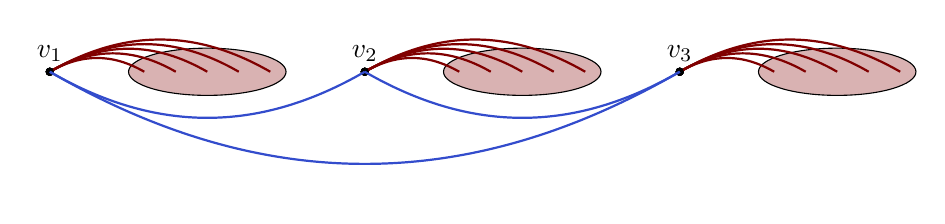
\begin{tikzpicture}
    \foreach \s in {0, 4, 8} {
      \begin{scope}[shift={(\s, 0)}]
        \node [circ] {};

        \draw [fill opacity=0.3, fill=mred] (2, 0) ellipse (1 and 0.3);
        \foreach \x in {1.2,1.6,2.0,2.4,2.8} {
          \draw (0, 0) edge [bend left, mred, thick] (\x, 0) node [circ] {};
        }
      \end{scope};
    }
    \draw (0, 0) edge [bend right, mblue, thick] (4, 0);
    \draw (4, 0) edge [bend right, mblue, thick] (8, 0);
    \draw (0, 0) edge [bend right, mblue, thick] (8, 0);
    \node at (0, 0) [above] {$v_1$};
    \node at (4, 0) [above] {$v_2$};
    \node at (8, 0) [above] {$v_3$};
  \end{tikzpicture}
\end{center}
But this argument is rather weak, because we didn't use that large pool of blue edges we've found at $v_1$. So in fact this time we can do better than $n^2$.
\begin{thm}
  We have
  \[
    R(3, n) \leq \frac{100 n^2}{\log n}
  \]
  for sufficiently large $n \in \N$.
\end{thm}
Here the $100$ is, obviously, just some random big number.

\begin{proof}
  Let $N \geq 100n^2/\log n$, and consider a red-blue colouring of the edges of $K_N$ with no red $K_3$. We want to find a blue $K_n$ in such a colouring.

  We may assume that
  \begin{enumerate}
    \item No vertex $v$ has $ \geq n$ red edges incident to it, as argued just now.
    \item If we have $v_1, v_2, v_3$ such that $v_1v_2$ and $v_1 v_3$ are red, then $v_2 v_3$ is blue:
      \begin{center}
        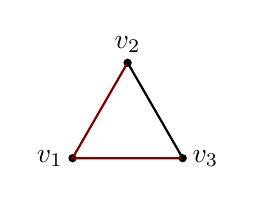
\begin{tikzpicture}[scale=0.7]
          \node [circ] at (0, 0) {};
          \node [circ] at (2, 0) {};
          \node [circ] at (1, 1.732) {};
          \draw [mred, thick] (2, 0) -- (0, 0) -- (1, 1.732);
          \draw [thick] (1, 1.732) -- (2, 0);

          \node [left] at (0, 0) {$v_1$};
          \node [above] at (1, 1.732) {$v_2$};
          \node [right] at (2, 0) {$v_3$};
        \end{tikzpicture}
      \end{center}
  \end{enumerate}
  We now let
  \[
    \mathcal{F} = \{\mathcal{U} : \mathcal{U} \subseteq V(K_N)\text{ such that }\mathcal{U}^{(2)} \text{ is monochromatic and blue}\}.
  \]
  We want to find some $\mathcal{U} \in \mathcal{F}$ such that $|\mathcal{U}| \geq n$, ie. a blue $K_n$. How can we go about finding this?

  Let $W$ be a uniformly random member of $\mathcal{F}$. We will be done if we can show that that $\E[|W|] \geq n$.

  We are going to define a bunch of random variables. For each vertex $v \in V(K_N)$, we define the variable
  \[
    X_v = n \mathbf{1}_{\{v \in W\}} + |\{u: uv\text{ is red and }u \in W\}|.
  \]
  \begin{claim}
   \[
    \E[X_v] > \frac{\log n}{10}
  \]
  for each vertex $v$.
  \end{claim}
  To see this, let
  \[
    A = \{u: uv \text{ is red}\}
  \]
  and let
  \[
    B = \{u: uv \text{ is blue}\}.
  \]
  then from the properties we've noted down, we know that $|A| < n$ and $A^{(2)}$ is blue. So we know very well what is happening in $A$, and nothing about what is in $B$.

  We fix a set $S \subseteq B$ such that $S \in \mathcal{F}$, ie. $S^{(2)}$ is blue. What can we say about $W$ if we condition on $B \cap W = S$?
  \begin{center}
    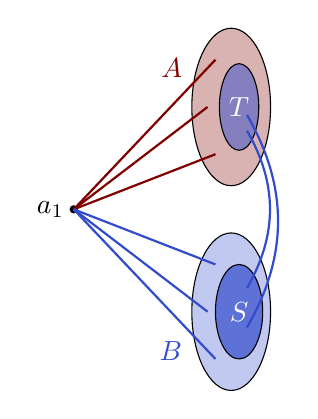
\begin{tikzpicture}
      \node [circ] {};
      \node [left] {$a_1$};

      \draw [fill opacity=0.3, fill=mred] (2, 1.3) ellipse (0.5 and 1);
      \draw [fill opacity=0.3, fill=mblue] (2, -1.3) ellipse (0.5 and 1);

      \draw [thick, mred] (0, 0) -- (1.8, 1.9);
      \draw [thick, mred] (0, 0) -- (1.7, 1.3);
      \draw [thick, mred] (0, 0) -- (1.8, 0.7);

      \draw [thick, mblue] (0, 0) -- (1.8, -1.9);
      \draw [thick, mblue] (0, 0) -- (1.7, -1.3);
      \draw [thick, mblue] (0, 0) -- (1.8, -0.7);

      \draw [fill=mblue, fill opacity=0.7] (2.1, -1.3) ellipse (0.3 and 0.6);

      \node at (2.1, -1.3) [white] {$S$};

      \node [mblue, left] at (1.5, -1.8) {$B$};
      \node [mred, left] at (1.5, 1.8) {$A$};

      \draw [fill=mblue, fill opacity=0.5] (2.1, 1.3) ellipse (0.25 and 0.55);

      \node at (2.1, 1.3) [white] {$T$};

      \draw (2.2, -1) edge [bend right, mblue, thick] (2.2, 1);
      \draw (2.2, -1.5) edge [bend right, mblue, thick] (2.2, 1.2);
    \end{tikzpicture}
  \end{center}
  Let $T \subseteq A$ be the set of vertices that are joined to $S$ only by blue edges. Write $|T| = x$. Then if $B \cap W = S$, then either $W \subseteq S \cup T$, or $W \subseteq S \cup \{v\}$. So there are exactly $2^x + 1$ choices of $W$. So we know
  \begin{align*}
    \E[X_v \mid W \cap B = S] &\geq \frac{n}{2^x + 1} + \frac{2^x}{2^x + 1}(\E[|\text{random subset of T}|])\\
    &= \frac{n}{2^x + 1} + \frac{2^{x - 1}x}{2^x + 1}.
  \end{align*}
  Now if
  \[
    x < \frac{\log n}{2},
  \]
  then
  \[
    \frac{n}{2^x + 1} \geq \frac{n}{\sqrt{n} + 1} \geq \frac{\log n}{10}
  \]
  for all sufficiently large $n$. On the other hand, if
  \[
    x \geq \frac{\log n}{2},
  \]
  then
  \[
    \frac{2^{x - 1}x}{2^x + 1} \geq \frac{1}{4} \cdot \frac{\log n}{2} \geq \frac{\log n}{10}.
  \]
  So we are done.

  \begin{claim}
    \[
      \sum_{v \in V} X_v \leq 2n |W|.
    \]
  \end{claim}
  To see this, for each vertex $v$, we know that if $v \in W$, then it contributes $n$ to the sum via the first term. Also, by our initial observation, we know that $v \in W$ has at most $n$ neighbours. So it contributes at most $n$ to the second term (acting as the ``$u$'').

  Finally, we know that
  \[
    \E[|W|] \geq \frac{1}{2n} \sum \E[X_V] \geq \frac{N}{2n} \frac{\log n}{10} \geq \frac{100n^2}{\log n} \cdot \frac{\log n}{20 n} \geq 5n.
  \]
  Therefore we can always find some $\mathcal{U} \in \mathcal{F}$ such that $|\mathcal{U}| \geq n$.
\end{proof}

Now of course, there is the following obvious generalization of Ramsey numbers:
\begin{defi}[$R(G, H)$]\index{$R(G, H)$}
  Let $G, H$ be graphs. Then we define $R(G, H)$ to be the smallest $N$ such that any red-blue colouring of $K_N$ has either a red copy of $G$ or a blue copy of $H$.
\end{defi}
Obviously, we have $R(G, H) \leq R(|G|, |H|)$. So the natural question is if we can do better than that.

\begin{ex}
  Show that
  \[
    R(P_n, P_n) \leq 2n.
  \]
\end{ex}
So sometimes it cna be much better.

\section{Ramsey theory on the integers}
So far, we've been talking about what happens when we finitely colour graphs. What if we $k$-colour the integers $\N$? What can we say about it?

It is a trivial statement that this colouring has a monochromatic subset, by the pigeonhole principle. Interesting questions arise when we try to take the additive structure of $\N$ into account. So we could ask, can we find a monochromatic ``copy'' of $\N$.

One way to make this question concrete is to ask if there is an infinite monochromatic arithmetic progression.

The answer is easily a ``no''! There are only countably many progressions, so for each arithmetic progression, we pick two things in the progression and colour them differently.

We can also construct this more concretely. We can colour the first number red, the next two blue, the next three red etc. then it is easy to see that it doesn't have an infinite arithmetic progression. % insert picture

But this is somewhat silly, because there is a significant amount of structure in the sequence there. It turns out the following is true:
\begin{thm}[van der Waerden theorem]\index{van der Waerden theorem}
  Let $m, k \in N$. Then there is some $N = W(m, k)$ such that whenever $[N]$ is $k$-coloured, then there is a monochromatic arithmetic progression of length $n$.
\end{thm}

The idea is to do induction on $m$. We will using colourings with much greater than $k$ colours to deduce the existence of $W(m, k)$.

We can try a toy example first. Let's try to show that $W(3, 2)$ exists. Suppose we have three natural numbers:
\begin{center}
  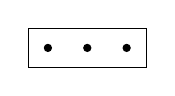
\begin{tikzpicture}[scale=0.5]
    \draw (-0.5, 0.5) rectangle (2.5, -0.5);
    \node [circ] at (0, 0) {};
    \node [circ] at (1, 0) {};
    \node [circ] at (2, 0) {};
  \end{tikzpicture}
\end{center}
By the pigeonhole principle, there must be two things that are the same colour, say
\begin{center}
  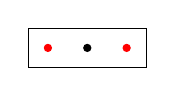
\begin{tikzpicture}[scale=0.5]
    \draw (-0.5, 0.5) rectangle (2.5, -0.5);
    \node [circ, red] at (0, 0) {};
    \node [circ] at (1, 0) {};
    \node [circ, red] at (2, 0) {};
  \end{tikzpicture}
\end{center}
If this is the case, then if we don't want to have an arithmetic progression of length $3$, then the fifth number must be blue
\begin{center}
  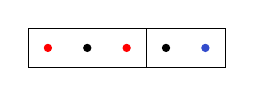
\begin{tikzpicture}[scale=0.5]
    \draw (-0.5, 0.5) rectangle (2.5, -0.5);
    \node [circ, red] at (0, 0) {};
    \node [circ] at (1, 0) {};
    \node [circ, red] at (2, 0) {};

    \draw (2.5, -0.5) rectangle (4.5, 0.5);
    \node [circ] at (3, 0) {};
    \node [circ, mblue] at (4, 0) {};
  \end{tikzpicture}
\end{center}
We now cut the universe into blocks into 5 things. Again by the pigeonhole principle, there must be two blocks that look the same. Say it's this block again.
\begin{center}
  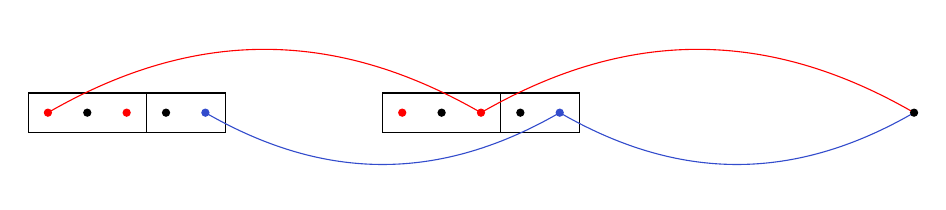
\begin{tikzpicture}[scale=0.5]
    \draw (-0.5, 0.5) rectangle (2.5, -0.5);
    \node [circ, red] at (0, 0) {};
    \node [circ] at (1, 0) {};
    \node [circ, red] at (2, 0) {};

    \draw (2.5, -0.5) rectangle (4.5, 0.5);
    \node [circ] at (3, 0) {};
    \node [circ, mblue] at (4, 0) {};

    \begin{scope}[shift={(9, 0)}]
      \draw (-0.5, 0.5) rectangle (2.5, -0.5);
      \node [circ, red] at (0, 0) {};
      \node [circ] at (1, 0) {};
      \node [circ, red] at (2, 0) {};

      \draw (2.5, -0.5) rectangle (4.5, 0.5);
      \node [circ] at (3, 0) {};
      \node [circ, mblue] at (4, 0) {};
    \end{scope}
    \draw [red] (0, 0) edge [bend left] (11, 0);
    \draw [red] (11, 0) edge [bend left] (22, 0);

    \draw [mblue] (4, 0) edge [bend right] (13, 0);
    \draw [mblue] (13, 0) edge [bend right] (22, 0);

    \node [circ] at (22, 0) {};
  \end{tikzpicture}

\end{center}
Now we have two sequences, and the point at the end belongs to both of the two sequences. And no matter what colour it is, we are done.

For $k = 3$, we can still find such a block, but now that third point could be a third colour, say, green. When then find these bigger blocks, and it must repeat, and then we are done again.

In the case $m = 2$, we used the pigeonhole principle. When we have $m > 2$, we will use van der Waerden theorem for smaller $m$ inductively.

We now come up with names to describe the scenario we had above.
\begin{defi}[Focused progression]\index{focused progression}
  We say a collection of arithmetic progressions $A_1, A_2, \cdots, A_r$ of length $m$ with
  \[
    A_i = \{a_i, a_i + d_i, \cdots, a_i + (m - 1) d_i\}
  \]
  are \emph{focused} at $f$ if $a_i + m d_i = f$ for all $1 \leq i \leq r$.
\end{defi}

\begin{eg}
  $\{1, 4\}$ and $\{5, 6\}$ are focused at $7$.
\end{eg}

\begin{defi}[Colour focused progression]\index{colour focused progression}\index{focus progression!colour}
  If $A_1, \cdots, A_r$ are focused at $f$, and each $A_i$ is monochromatic and no two are the same colour, then we say they are \emph{colour focused} at $f$.
\end{defi}

We can now write the proof
\begin{proof}
  We induct on $m$. The result is clearly trivial when $m = 1$, and follows easily from the pigeonhole principle when $m = 2$.

  Suppose $m > !$, and assume inductively that $W(m - 1, k')$ exists for any $k' \in \N$.

  Here is the claim we are trying to established:
  \begin{claim}
    For each $r \leq k$, there is a natural number $n$ such that whenever we $k$-colour $[n]$, then either
    \begin{enumerate}
      \item There exists a monochromatic AP of length $m$; or
      \item There are $r$ colour-focused AP's of length $m - 1$.
    \end{enumerate}
  \end{claim}
  It is clear that this claim implies the theorem, as we can pick $r = k$. Then if there isn't a monochromatic AP of length $m$, then we look at the colour of the common focus, and it must be one of the colours of those AP's.

  To prove the claim, we induct on $r$. When $n = 1$, we may take $W(m - 1, k)$. Now suppose $r > 1$, and some $n'$ works for $r - 1$. With the benefit of hindsight, we shall show that
  \[
    n = W(m - 1, k^{2n'}) 2n'
  \]
  works for $r$.

  We consider any $k$-colouring of $[n]$, and suppose it has no monochromatic AP of length $m$. We need to find $r$ colour-focused progressions of length $n - 1$.

  We view this $k$-colouring of $[n]$ as a $k^{2n'}$ colouring of blocks of length $2n'$, of which there are $W(m - 1, k^{2n'})$.

  Then by definition of $W(m - 1, k^{2n'})$, we can find blocks
  \[
    B_s, B_{s + t}, \cdots, B_{s + (m - 2)t}
  \]
  which are coloured identically. By the inductive hypothesis, we know each $B_s$ contains $r - 1$ colour-focused AP's of length $m - 1$, say $A_1, .., A_{r - 1}$ with first terms $a_1, \cdots, a_r$ and common difference $d_1 , \cdots, d_{r - 1}$, and also their focus $f$, because the length of $B_s$ is $2n'$, not just $n'$.

  Since we assumed there is no monochromatic progression of length $n$, we can assume $f$ has a different colour than the $A_i$.

  Now consider $A_1', A_2', \cdots, A_{r - 1}'$, where $A_i'$ has first term $a_i$, common difference $d_i + 2n't$, and length $m - 1$. This difference sends us to the next block, and then the next term in the AP. We also pick $A_r'$ to consist of the all the focus of the blocks $B_i$, namely
  \[
    A_r' = \{f, f + 2n't, \cdots, f + 2n't(m - 2)\}
  \]
  These progressions are monochromatic with distinct colours, and focused at $f + (2n' t)(m - 1)$. So we are done.
\end{proof}

This argument, where one looks at the induced colourings of blocks, is called a \term{product argument}.

The bounds we obtain from this argument is, as one would expect, terrible. We have
\[
  W(3, k) \leq k^{\iddots^k}, % check
\]
where the tower of $k$'s has length $k$.

Instead of an arithmetic progression, why don't we ask for something that looks like $\{d, 2d, 3d, \cdots, nd\}$? This is answered on the example sheet.

Now we can generalize in a different way. What can we say about monochromatic structures a $k$-colouring of $\N^d$? What is the right generalization of van der Waerden theorem?

To figure out the answer, we need to find the right generalization of arithmetic progressions.

\begin{defi}[Homothelic copy]\index{homothelic copy}
  Given a finite $S \subseteq \N^d$, a \emph{homothetic copy} of $S$ is a set of the form
  \[
    \ell S + \mathcal{M},
  \]
  where $\ell, \mathcal{M} \in \N^d$ and $\ell \not= 0$.
\end{defi}

\begin{eg}
  An arithmetic progression of length $m$ is just a homothetic copy of $[m] = \{1, 2, \cdots, m\}$.
\end{eg}

Thus, the theorem we want to say is the following:
\begin{thm}[Gallai]
  Whenever $\N^d$ is $k$-coloured, there exists a monochromatic (homothetic) copy of $S$ for each finite $S \subseteq \N^d$.
\end{thm}

In order to prove this, we prove the beautiful Hales--Jewett theorem, which is in some sense the abstract core of the argument we used for van der Waerden theorem.

We need a bit of set up. As usual, we write
\[
  [m]^n = \{(x_1, \cdots, x_n): x_i \in [m]\}.
\]
Here is the important definition:
\begin{defi}[Combinatorial line]\index{combinatorial line}
  A \emph{combinatorial line} $L \subseteq [m]^n$ is a set of the form
  \[
    \{(x_1, \cdots, x_nn): x_i = x_j\text{ for all }i, j \in I; x_i = a_i\text{ for all }i \not\in I\}
  \]
  for some fixed non-empty set of coordinates $I \subseteq [n]$ and $a_i \in [m]$.

  $I$ is called the set of \term{active coordinates}.
\end{defi}

\begin{eg}
  Here is a line in $[3]^2$
  \begin{center}
    \begin{tikzpicture}
      \foreach \x in {0, 1, 2} {
        \foreach \y in {0, 1, 2} {
          \node [circ] at (\x, \y) {};
        }
      }
      \draw (0, 0) -- (0, 2);
    \end{tikzpicture}
  \end{center}
  Ths line is given by $I = \{1\}$, $a_2 = 1$.

  The following shows all the lines we have:
  \begin{center}
    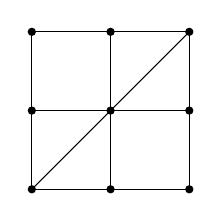
\begin{tikzpicture}
      \foreach \x in {0, 1, 2} {
        \foreach \y in {0, 1, 2} {
          \node [circ] at (\x, \y) {};
        }
      }
      \foreach \x in {0, 1, 2} {
        \draw (\x, 0) -- (\x, 2);
        \draw (0, \x) -- (2, \x);
      }
      \draw (0, 0) -- (2, 2);
    \end{tikzpicture}
  \end{center}
\end{eg}
It is easy to see that any line has exactly $[m]$ elements. We write $L^-$ and $L^+$ for the first and last point of the line, ie. the points where the active coordinates are all $1$ and $m$ respectively. Note that it is clear that any line $L$ is uniquely determined by $L^-$ and its active coordinates.

\begin{eg}
  In $[3]^3$, we have the line
  \[
    L = \{(1, 2, 1), (2, 2, 2), (3, 2, 3)\}.
  \]
  This is a line with $I = \{1, 3\}$ and $a_2 = 2$. The first and last points are $(1, 2, 1)$ and $(3, 2, 3)$.
\end{eg}

\begin{thm}[Hales--Jewett theorem]\index{Hales--Jewett theorem}
  For all $m, k \in \N$, there exists $N = HJ(m, k)$ such that whenever $[m]^N$ is $k$-coloured, there exists a monochromatic line.
\end{thm}
Note that this theorem implies van der Waerden's theorem easily. The idea is to embed $[m]^N$ into $\N$ linearly, so that a monochromatic line in $[m]^N$ gives an arithmetic progression of length $m$. Explicitly, given a $k$-colouring $c: \N \to [k]$, we define $c': [m]^N \to [k]$ by
\[
  c'(x_1, x_2, \cdots, x_N) = c(x_1 + x_2 + \cdots + x_N).
\]
Now a monochromatic line gives us an arithmetic progression of length $m$. For example, if the line is
\[
  L = \{(1, 2, 1), (2, 2, 2), (3, 2, 3)\},
\]
then we get the monochromatic progression $4, 6, 8$ of length $3$. In general, the monochromatic AP defined has $d = |I|$.

The proof is essentially what we did for van der Waerden theorem. We are going to build a lot of almost-lines that point at the same vertex, and then no matter what colour the last vertex is, we are happy.

\begin{defi}[Focused lines]\index{focused lines}
  We say lines $L_1, \cdots, L_r$ are \emph{focused} at $f \in [m]^N$ if $L_i^+ = f$ for all $i = 1, \cdots, r$.
\end{defi}

\begin{defi}[Colour focused lines]\index{colour focused lines}\index{focused lines!colour}
  If $L_1, \cdots, L_r$ are focused lines, and $L_i \setminus \{L_i^+\}$ is monochromatic for each $i = 1, \cdots, r$ and all these colours are distinct, then we say $L_1, \cdots, L_r$ are \emph{colour focused} at $f$.
\end{defi}

The proof is just like the proof of van der Waerden theorem.
\begin{proof}
  We proceed by induction on $m$. This is clearly trivial for $m = 1$, as a line only has a single point.

  Now suppose $m > 1$, and that $HJ(m - 1, k)$ exists for all $k \in \N$. As before, we will prove the following claim:
  \begin{claim}
    For each $1 \leq r \leq k$, there is an $n \in \N$ such that in any $k$-colouring of $[m]^n$, either
    \begin{enumerate}
      \item there exists a monochromatic line; or
      \item there exists $r$ colour-focused lines.
    \end{enumerate}
  \end{claim}
  Again, the result is immediate from the claim, as we just use it for $r = k$ and look at the colour of the focus.

  The prove this claim, we induct on $r$. If $r = 1$, then picking $n = HJ(m - 1, k)$ works, as a single colour-focused line of length $n$ is just a monochromatic line of length $n - 1$, and $[m - 1]^n \subseteq [m]^n$ naturally.

  Now suppose $r > 1$ and $n$ works for $r - 1$. Then we will show that $n + n'$ works, where
  \[
    n' = HJ(m - 1, k^{m^n}).
  \]
  Consider a colouring $c: [m]^{n + n'} \to [k]$, and we assume this has no monochromatic lines.

  We think of $[m]^{n + n'}$ as $[m]^n \times [m]^{n'}$. So for each point in $[m]^{n'}$, we have a whole cube $[m]^n$. Consider a $k^{m^n}$ colouring of $[m]^{n'}$ as follows --- given any $x \in [m]^{n'}$, we look at the subset of $[m]^{n + n'}$ containing the points with last $n'$ coordinates $x$. Then we define the new colouring of $[m]^{n'}$ to be the restriction of $c$ to this $[m]^n$, and there are $m^n$ possibilities.

  Now there exists a line $L$ such that $L \setminus L^+$ is monochromatic for the new colouring. This means for all $a \in [m]^n$ and for all $b, b' \in L\setminus L^+$, we have
  \[
    c(a, b) = c(a, b').
  \]
  Let $c''(a)$ denote this common colour for all $a \in [m]^n$. this is a $k$-colouring of $[m]^n$ with no monochromatic line (because $c$ doesn't have any). So by definitoin of $n$, there exists lines $L_1, L_2, \cdots, L_{r - 1}$ in $[m]^n$ which are colour-focused at some $f \in [m]^n$ for $c''$.

  In the proof of van der Waerden, we had a progression within each block, and also how we just between blocks. Here we have the same thing. We have the lines in $[m]^n$, and also the ``external'' line $L$.
  \begin{center}
    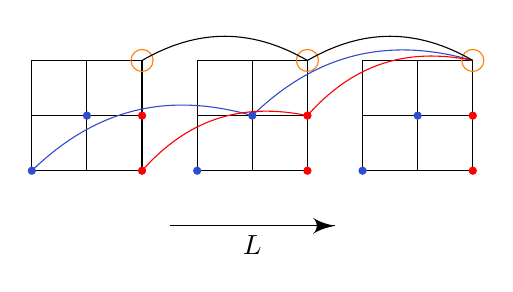
\begin{tikzpicture}[scale=0.7]
      \foreach \x in {0, 3, 6}{
        \begin{scope}[shift={(\x, 0)}]
          \draw [step=1] (0, 0) grid (2, 2);

          \node [circ, mblue] at (0, 0) {};
          \node [circ, mblue] at (1, 1) {};
          \node [circ, red] at (2, 0) {};
          \node [circ, red] at (2, 1) {};

          \draw [morange] (2, 2) circle [radius=0.2];
        \end{scope}
      }

      \draw [->] (2.5, -1) -- (5.5, -1) node [pos=0.5, below] {$L$} ;

      \draw [mblue] (0, 0) edge [bend left] (4, 1);
      \draw [mblue] (4, 1) edge [bend left] (8, 2);

      \draw [red] (2, 0) edge [bend left] (5, 1);
      \draw [red] (5, 1) edge [bend left] (8, 2);
      \draw (2, 2) edge [bend left] (5, 2);
      \draw (5, 2) edge [bend left] (8, 2);
    \end{tikzpicture}
  \end{center}
  Consider the line $L_1', L_2', \cdots, L_{r - 1}'$ in $[m]^{n + n'}$, where
  \[
    L_i' = (L_i^-, L^-),
  \]
  and the active coordiante set is $I_i \cup I$, where $I$ is the active coordiante set of $L$.

  Also consdier the line $F$ with $F^- = (f, L^-)$ and active coordinate set $I$.

  Then we see that $L_1', \cdots, L_{r - 1}', F$ are $r$ colour-focused lines with focus $(f, L^+)$.
\end{proof}

We can now prove our generalized van der Waerden.
\begin{thm}[Gallai]
  Whenever $\N^d$ is $k$-coloured, there exists a monochromatic (homothetic) copy of $S$ for each finite $S \subseteq \N^d$.
\end{thm}

\begin{proof}
  Let $S = \{S(1), S(2), \cdots, S(m)\} \subseteq \N^d$. Given a $k$-colouring $\N^d \to [k]$, we induce a $k$-colouring $c: [m]^N \to [k]$ by
  \[
    c'(x_1, \cdots, x_N) = c(S(x_1) + S(x_2) + \cdots + S(x_N)).
  \]
  By Hales-Jewett, for sufficiently large $N$, there exists a monochromatic line $L$ for $c'$, which gives us a monochromatic homothetic copy of $S$ in $\N^d$. For example, if the line is $(1\; 2\; 1)$, $(2\; 2\; 2)$ and $(3\; 2\; 3)$, then we know
  \[
    c(S(1) + S(2) + S(1)) = c(S(2) + S(2) + S(2)) = c(S(3) + S(2) + S(3)).
  \]
  So we have the monochromatic homothetic copy $\lambda S + \mu$ , where $\lambda = 2$ (the number of active coordinates), and $\mu = S(2)$.
\end{proof}

\subsection{Largeness in Ramsey theory*}
We say $X \subseteq \N^{(2)}$ is \emph{large} if $X$ contains an infinite complete graph. Then Ramsey's theorem says if we finitely colour $\N$, then one of the colours gives a large subset.

We say a $X \subseteq \N$ is large if $X$ contains an $m$ AP for all $m \in \N$. Again van der Waerden says if we finitely colour $\N$, then there is one colour that gives a large subset.

But if we are lazy, then we might try to find such a large set simply by looking at the ``largest'' subset. So one natural question is as follows --- does a simpler ``counting'' notion of largeness imply Ramsey-theoretic structures?

In $\N^{(2)}$ the answer is no, as there isn't much structure in $\N^{(2)}$, so we can only talk about whether things are infinite or not.

However, in $\N$, we can talk about density.
\begin{defi}[Density]
 For $A \subseteq \N$, we let the \term{density} of $A$ as
 \[
   \bar{d}(A) = \limsup_{(b - a) \to \infty} \frac{A \cap [a, b]}{|b - a|}.
 \]
\end{defi}
Clearly, in any finite $k$-colouring of $\N$, there exists a colour class with positive density.

Thus, we want to know if a positive density implies the existence of progressions. Remarkably, the answer is yes!
\begin{thm}[Szemer\'edi theorem]\index{Szemer\'edi theorem}
  Let $\delta > 0$ and $m \in \N$. Then there exists some $N = S(m, \delta) \in \N$ such that any subset $A \subseteq [N]$ with $|A| \geq \delta N$ contains an $m$-term arithmetic progression.
\end{thm}
The proof of this theorem is usually the subject of an entire lecture course, so we are not going to attempt to prove this. Even the particular case $m = 3$ is very hard.

This theorem has a lot of very nice Ramsey consequences. In the case of graph colourings, we asked ourselves what happens if we colour a graph with \emph{infinitely} many colours. Suppose we now have a colouring $c: \N \to \N$. Can we still find a monochromatic progression of length $m$? Of course not, because $c$ can be injective.

\begin{thm}
  For any $c: \N \to \N$, there exists a $m$-AP on which either
  \begin{enumerate}
    \item $c$ is constant; or
    \item $c$ is injective.
  \end{enumerate}
\end{thm}
It is also possible to prove this directly, but it is easy with the previous theorem.

\begin{proof}
  We set
  \[
    \delta = \frac{1}{m^2(m + 1)^2}.
  \]
  We let $N = S(m, \delta)$. We write
  \[
    [N] = A_1 \cup A_2 \cup \cdots \cup A_k,
  \]
  where the $A_i$'s are the colour-classes of $c|_{[N]}$. By choice of $N$, we are done if $|A_i| \geq \delta N$ for some $1 \leq i \leq k$. So suppose not.

  Let's try to count the number of arithmetic progressions in $[N]$. There are more than $N^2/(m + 1)^2$ of these, as we can take any $a, d \in [N/m + 1]$. We want to show that there is an AP that hits each $A_i$ at most once.

  Next, we count the number of AP's that hits $A_i$ at least twice. We need to pick two terms in $A_i$, and also decide which two terms in the progression they are in, eg. they can be the first and second term, or the 5th and 17th term. So there are at most $m^2 |A_i|^2$ terms.

  So the number of AP's on which $c$ is injective is greater than
  \[
    \frac{N^2}{(m + 1)^2} - k |A_i|^2 m^2 \geq \frac{N^2}{(m + 1)^2} - \frac{1}{\delta} (\delta N)^2 m^2 = \frac{N^2}{(m + 1)^2} - \delta N^2 m^2 \geq 0.
  \]
  So we are done. Here the first inequality follows from the fact that $\sum |A_i| = [N]$ and each $|A_i| < \delta N$.
\end{proof}

Now let's look at a colouring $c: \N^{(2)} \to [2]$ again. As before, we say a set $X$ is monochromatic if $c|_{X^{(2)}}$ is constant. Now we want to try to find a monochromatic set with some arithmetic properties.

The first question we ask is --- can we find a monochromatic 3-term arithmetic progression? The answer is no --- we define $c(ij)$ to be the parity of largest power of $2$ dividing $j - i$.

What if we make some concessions --- can we find a blue 10-AP, or if not, say, that red has an infinite set? The answer is again no. We can make progressively larger red cliques, and take all other edges blue. If we double the size of the red cliques every time, it is not hard to check that there is no blue 4-AP, and no infinite red set.
\begin{center}
  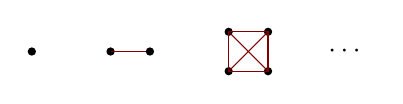
\begin{tikzpicture}
    \node [circ] at (0, 0) {};

    \node [circ] at (1, 0) {};
    \draw [mred] (1, 0) -- (1.5, 0);
    \node [circ] at (1.5, 0) {};

    \node [circ] at (2.5, 0.25) {};
    \node [circ] at (3, 0.25) {};
    \node [circ] at (2.5, -0.25) {};
    \node [circ] at (3, -0.25) {};

    \draw [mred] (2.5, 0.25) -- (2.5, -0.25) -- (3, -0.25) -- (3, 0.25) -- cycle;

    \draw [mred] (2.5, 0.25) -- (3, -0.25);
    \draw [mred] (2.5, -0.25) -- (3, 0.25);

    \node at (4, 0) {$\cdots$};
  \end{tikzpicture}
\end{center}
What if we further relax our condition, and only require an arbitrarily large red set?
\begin{thm}
  For any $c: \N^{(2)} \to \{\mathrm{red}, \mathrm{blue}\}$, either
  \begin{enumerate}
    \item There exists a blue $m$-AP for each $m \in \N$; or
    \item There exists arbitrarily large red sets.
  \end{enumerate}
\end{thm}

\begin{proof}
  Suppose we can't find a blue $m$-AP for some fixed $m$. We induct on $r$, and try to find a red set of size $r$.

  Say $A \subseteq \N$ is a progression of length $N$. Since $A$ has no blue $m$-term progression, so it must contain many red edges. Indeed, each $m$-AP in $A$ must contain a red edge. Also each edge specifies two points, and this can be extended to an $m$-term progression in at most $m^2$ ways. Since there are $N^2/(m + 1)^2$. So there are at least
  \[
    \frac{N^2}{m^2(m + 1)^2}
  \]
  red edges. With the benefit of hindsight, we set
  \[
    \delta = \frac{1}{2m^2(m + 1)^2}.
  \]
  The idea is that since we have lots of red edges, we can try to find a point with a lot of red edges connected to it, and we hope to find a progression in it.

  We say $X, Y \subseteq \N$ form an $(r, k)$-structure if
  \begin{enumerate}
    \item They are disjoint
    \item $X$ is red;
    \item $Y$ is an arithmetic progression;
    \item all $X\mdash Y$ edges are red;
    \item $|X| = r$ and $|Y| = k$.
  \end{enumerate} % insert a picture
  We show by induction that there is an $(r, k)$-structure for each $r$ and $k$.

  A $(1, k)$ structure is just a vertex connected by red edges to a $k$-point structure. If we take $N = S(\delta, k)$, we know among the first $N$ natural numbers, there are at least $N^2/(m^2(m + 1)^2)$ red edges inside $[N]$. So in particular, some $v \in [N]$ has at least $\delta N$ red neighbours in $[N]$, and so we know $v$ is connected to some $k$-AP by red edges. That's the base case done.

  Now suppose we can find an $(r - 1, k')$-structure for all $k' \in \N$. We set
  \[
    k' = S\left(\frac{1}{2m^2(m + 1)^2},, k\right).
  \]
  We let $(X, Y)$ be an $(r - 1, k')$-structure. As before, we can find $v \in Y$ such that $v$ has $\delta|Y|$ red neighbours in $Y$. Then we can find a progression $Y'$ of length $k$ in the red neighbourhood of $v$, and we are done, as $(X \cup \{v\}, Y')$ is an $(r, k)$-structure, and an ``arithmetic progression'' within an arithmetic progression is still an arithmetic progression.
\end{proof}
Before we end this chapter, we make a quick remark. Everything we looked for in this chapter involved the additive structure of the naturals. What about the multiplicative structure? For example, given a finite colouring of $\N$, can we find a monochromatic geometric progression? The answer is trivially yes. We can look at $\{2^x: x \in \N\}$, and then multiplication inside this set just looks like addition in the naturals.

But what if we want to mix additive and multiplicative structures? For example, can we always find a monochromatic set of the form $\{x + y, xy\}$? Of course, there is the trivial answer $x = y = 2$, but is there any other? This question was answered positively in 2016! We will return to this later on.

\section{Partition Regularity}
\begin{defi}[Partition regularity]\index{partition regular}
  We say an $m \times n$ matrix $A$ over $\Q$ is \emph{partition regular} if whenever $\N$ is finitely coloured, there exists an $x \in \N^n$ such that $Ax = 0$ and $x$ is monochromatic, ie. all coordinate of $x$ have the same colour.
\end{defi}
We will write \term{W$\N$FC} to mean ``whenever $\N$ is finitely coloured''. Note that by scaling $A$, we may wlog $A$ is in fact a matrix of $\Z$. Unless otherwise specified, we will assume that $A$ has entries in $\Z$.

\begin{eg}[Schur's theorem]\index{Schur's theorem}
  Whenever $\N$ is finitely coloured, there exists a monochromatic set of the form $\{x, y, x + y\}$. In other words the matrix $\begin{pmatrix}1 & 1 & -1\end{pmatrix}$ is partition regular, since
  \[
    \begin{pmatrix}
      1 & 1 & -1
    \end{pmatrix}
    \begin{pmatrix}
      x\\y\\z
    \end{pmatrix} = 0 \Longleftrightarrow z = x + y.
  \]
\end{eg}

\begin{eg}
  How about $\begin{pmatrix}2 & 3 & -5\end{pmatrix}$. This is partition regular, because for any $x$, we have
  \[
    \begin{pmatrix}
      2 & 3 & -5
    \end{pmatrix}
    \begin{pmatrix}
      x\\x\\x
    \end{pmatrix} = 0.
  \]
\end{eg}

How about van der Waerden's theorem?
\begin{eg}
  Van der Waerden's theorem says there is a monochromatic $3$-AP $\{x_1, x_2, x_3\}$ whenever $\N$ is finitely-coloured. We know $x_1, x_2, x_3$ forms a $3$-AP iff
  \[
    x_3 - x_2 = x_2 - x_1,
  \]
  or equivalently
  \[
    x_3 + x_1 = 2 x_2.
  \]
  This implies that $\begin{pmatrix}1 & -2 & 1\end{pmatrix}$ is partition regular, but this is not very interesting since we can take $x_1 = x_2 = x_3$.

  It turns out we can find a set of the form $\{d, a, a + d, a + 2d, \cdots, a + md\}$ whenever $\N$ is finitely-coloured. This is on the second example sheet. By including this variable, we can write down the property of being a progression in a non-trivial format by
  \[
    \begin{pmatrix}
      1 & 1 & 0 & -1\\
      2 & 1 & 0 & -1
    \end{pmatrix}
    \begin{pmatrix}
      d \\ a \\ x_2 \\ x_3
    \end{pmatrix} = 0
  \]
  This obviously generalizes to an arbitrary $m$-AP.
\end{eg}
We've seen three examples of partition regular matrices. Of course, not every matrix is partition regular. The matrix $\begin{pmatrix}1 & 1\end{pmatrix}$ is not partition regular, for the silly reason that two positive things cannot add up to zero.

Let's now look at some non-trivial first matrix that is not partition regular.
\begin{eg}
  The matrix $\begin{pmatrix}2 & -1\end{pmatrix}$ is not partition regular, since we can put $c(x) = (-1)^n$, where $n$ is the maximum integer such that $2^n \mid x$. Then $\{x, 2x\}$ is never monochromatic.

  A similar argument shows that if $\lambda \in \Q$ is such that $\begin{pmatrix}\lambda, -1\end{pmatrix}$ is partition regular, then $\lambda = 1$.
\end{eg}
But if we write down a random matrix, say $\begin{pmatrix}2 & 3 & -6\end{pmatrix}$? The goal of this chapter is to find a complete characterization of matrices that are partition regular.

\begin{defi}[Columns property]\index{columns property}
  Let
  \[
    A =
    \begin{pmatrix}
      \uparrow & \uparrow & & \uparrow\\
      c^{(1)} & c^{(2)} & \cdots & c^{(n)}\\
      \downarrow & \downarrow & & \downarrow
    \end{pmatrix}.
  \]
  We say $A$ has the \emph{columns property} if there is a partition $[n] = B_1 \cup B_2 \cup \cdots \cup B_d$ such that
  \[
    \sum_{i \in B_s} c^{(i)} \in \spn\{c^{(i)} : c^{(i)} \in B_1 \cup \cdots \cup B_{s - 1}\}
  \]
  for $s = 1, \cdots, d$. In particular,
  \[
    \sum_{i \in B_1} c^{(i)} = 0
  \]
\end{defi}
What does this mean? Let's look at the matrices we've seen so far.
\begin{eg}
  $\begin{pmatrix}1 & 1 & -1\end{pmatrix}$ has the columns property by picking $B_1 = \{1, 3\}$ and $B_2 = \{2\}$.
\end{eg}

\begin{eg}
  $\begin{pmatrix}2 & 3 & -5\end{pmatrix}$ has the columns property by picking $B_1 = \{1, 2, 3\}$.
\end{eg}

\begin{eg}
  The matrix
  \[
    \begin{pmatrix}
      1 & 1 & -1 & 0 & 0 & \cdots & 0\\
      1 & 2 & 0 & -1 & 0 & \cdots & 0\\
      1 & 3 & 0 & 0 & -1 & \cdots & 0\\
      \vdots & \vdots & \vdots & \vdots & \vdots & \ddots & \vdots\\
      1 & m & 0 & 0 & 0 & \cdots & -1
    \end{pmatrix}
  \]
  has the column property. Indeed, we take $B_1 = \{1, 3, \cdots, m + 2\}$, and since $\{c^{(3)}, \cdots, c^{(m + 2)}\}$ spans all of $\R^m$, we know picking $B_2 = \{2\}$ works.
\end{eg}

\begin{eg}
  $\begin{pmatrix}\ell & -1\end{pmatrix}$ has the columns property iff $\ell = 1$.
\end{eg}

\begin{eg}
  $\begin{pmatrix}1 & 1 \end{pmatrix}$ does not have a columns property.
\end{eg}

The goal of this chapter is to prove the following:
\begin{thm}[Rado]\index{Rado's theorem}
  A matrix $A$ is partition regular iff it has the column property.
\end{thm}
This is a remarkable theorem! The property of being partition regular involves a lot of quantifiers, over infinitely many things, but the column property is entirely finite, and we can get a computer to check it for us easily.

Another remarkable property of this theorem is that neither direction is obvious! It turns out partition regularity implies the column property is (marginally) easier, because if we know something is partition regular, then we can try to cook up some interesting colourings and see what happens. The other direction is harder.

To get a feel of the result, we will first prove it in the case of a single equation. The columns property in particular becomes much simpler. It just means that there exists a non-empty subset of the non-zero $a_i$'s that sums up to zero.

\begin{thm}
  If $a_1,\cdots, a_n \in \Q$, then $\begin{pmatrix} a_1 & \cdots & a_n \end{pmatrix}$ is partition regular iff there exists a non-empty $I \subseteq [n]$ such that
  \[
    \sum_{i \in I} a_i = 0.
  \]
\end{thm}

\section{Topological Dynamics}

\printindex
\end{document}
